% !TEX encoding = UTF-8
% !TEX TS-program = pdflatex
% !TEX root = ../Tesi.tex
% !TEX spellcheck = en-EN

%************************************************
\chapter[Experimental Characterization]{Experimental Characterization}
\chaptermark{Experimental}
\label{cap:experimentalcharacterization}
%************************************************

In the industrial processes we presented in Chapter \ref{cap:insufficiency} and
in Part \ref{par:applications} the following materials:
\begin{itemize}
  \item{coke,}
  \item{iron ore,}
  \item{limestone,}
  \item{sinter,} 
\end{itemize}
are involved, which can be furtherly divided according to the diameter of the
particles in two categories:
\begin{itemize}
  \item{fine, until 3.15 millimiters;}
  \item{coarse, larger than 3.15 millimiters.}
\end{itemize}

We followed a series of standardized procedures to characterize these particles,
as explained by various authors (\citet{RefWorks:45, RefWorks:46}).
These experimental data were later used to determine \acs{DEM} numerical
parameters, as explained in Chapters \ref{cap:numericalsimulation} and
\ref{cap:anntraining}.\\
For our investigations we focused on particle-particle (\acs{pp}) interactions,
and the bulk behaviour representative values summarized in Table
\ref{tab:14bulkvalues}.
According to \citet{RefWorks:136}, they are the most relevant for the large,
dense conditions we researched.

\begin{table}[h]
  \centering
    \begin{tabular}{lcc}
    \hline
     & acronym & formula \\ 
     \hline
    bulk density & \ac{rhob} & $\frac{mass ~ of ~ the ~ bulk}{volume ~ of ~ the ~ bulk}$ \\ 
    [5pt]
     
    steady-state flow/pre-shear coefficient of internal friction & \ac{mupsh}
     & $\frac{\tau_{psh}}{\sigma_{n,psh}}$ \\      [5pt]
     
    incipient flow/shear coefficient of internal friction & \ac{mush} &
    $\frac{\tau_{sh}}{\sigma_{n,sh}}$ \\      [5pt]
     
    static angle of repose & \ac{AoR}   & from the slope \\
\hline
    
    \end{tabular}%
  \caption{Values representative of bulk behaviour.}
\label{tab:14bulkvalues}
\end{table}%


\section{Particle Distribution}
\label{sec:particledistribution}

Determine the particles distribution is the first task in bulk materials
characterization, see \citet{RefWorks:44}.
Thus, we sieved each material investigated with an electrically tilting siever.
We proceded in a sequence from the largest to the smallest sieving diameter
(6.3, 5.6, 3.55, 2, 1.6, 1.25, 1, 0.8, 0.63, 0.5, 0.315, 0.25, 0.0001
millimiters). The results can be seen in Table
\ref{tab:19particlesizedistributions}.
\begin{sidewaystable}%[h]
\centering
\begin{tabular}{l|rccccccccccccc}
\hline
          & \multicolumn{1}{c}{Diameter [mm]} & 6.3   & 5.6   & 3.55  & 2     & 1.6   & 1.25  & 1     & 0.8   & 0.63  & 0.5   & 0.315 & 0.25  & 0.00001 \\
\hline
    coke  & \multicolumn{1}{l}{coarse} & 0.086 & 0.136 & 0.625 & 0.087 & 0.000 & 0.000 & 0.066 & 0.000 & 0.000 & 0.000 & 0.000 & 0.000 & 0.000 \\
    coke  & \multicolumn{1}{l}{fine} & 0.000 & 0.000 & 0.000 & 0.084 & 0.089 & 0.077 & 0.070 & 0.074 & 0.077 & 0.098 & 0.139 & 0.065 & 0.226 \\
    iron ore & \multicolumn{1}{l}{coarse} & 0.101 & 0.119 & 0.520 & 0.260 & 0.000 & 0.000 & 0.000 & 0.000 & 0.000 & 0.000 & 0.000 & 0.000 & 0.000 \\
    iron ore & \multicolumn{1}{l}{fine} & 0.000 & 0.000 & 0.000 & 0.354 & 0.175 & 0.149 & 0.129 & 0.063 & 0.051 & 0.032 & 0.017 & 0.029 & 0.000 \\
    limestone & \multicolumn{1}{l}{coarse} & 0.035 & 0.049 & 0.500 & 0.416 & 0.000 & 0.000 & 0.000 & 0.000 & 0.000 & 0.000 & 0.000 & 0.000 & 0.000 \\
    limestone & \multicolumn{1}{l}{fine} & 0.000 & 0.000 & 0.000 & 0.175 & 0.139 & 0.098 & 0.091 & 0.075 & 0.067 & 0.061 & 0.097 & 0.036 & 0.161 \\
    sinter & \multicolumn{1}{l}{coarse} & 0.061 & 0.100 & 0.709 & 0.096 & 0.000 & 0.000 & 0.034 & 0.000 & 0.000 & 0.000 & 0.000 & 0.000 & 0.000 \\
    sinter & \multicolumn{1}{l}{fine} & 0.000 & 0.000 & 0.000 & 0.454 & 0.157 & 0.103 & 0.226 & 0.028 & 0.031 & 0.000 & 0.000 & 0.000 & 0.000 \\
    
\hline
\end{tabular}
\caption[aaaValid DEM values]{aaaValid DEM values. For each parameter we show
the valid parameter statistics in the two tests and in their intersection.
Finally, we show the number of valid parameter combinations over the total
(6250000).}
\label{tab:19particlesizedistributions}
\end{sidewaystable}

\section{Drained angle of repose (p-p) - small scale}
\label{sec:aor}

Later, we performed \acs{pp} drained angle of repose (\acs{AoR}) tests.
Drained, because each sample was completely dry and moistless.
\citet{RefWorks:69} defines \textit{angle of repose} the angle of the slope of a
bulk material sample when it reaches steady-state after deposition.\\
In our test, a sample was deposited on a 20 centimeters diameter plate (hence,
small scale) with liftable boundary called static \acs{AoR} tester, see Fig.
\ref{fig:088aorexperimental}.
Once the particles were in position, the boundary was lifted, allowing some
particles to drop.
Once stabilized, the \acs{AoR} was measured eight times using a digital
protractor at different positions of the heap.
The average of the measurements gave the fourth bulk value (see Table
\ref{tab:14bulkvalues}).
Note that, since the experiments were performed only for relatively large size
bulk solids, the compaction condition in the initial state was not critical to the
final result of this test.\\
In Table \ref{tab:23aor} the results of the tests performed on the various
materials can be seen.
\begin{figure}[htbp]
\centering 
  \subfloat[Drained angle of repose.]{
	  \includegraphics[width=.54\columnwidth]{images/051aorLab}
	  \label{fig:051aorLab}
  }
  \quad
    \subfloat[Drained angle of repose tester \cite{RefWorks:69}.]{
	  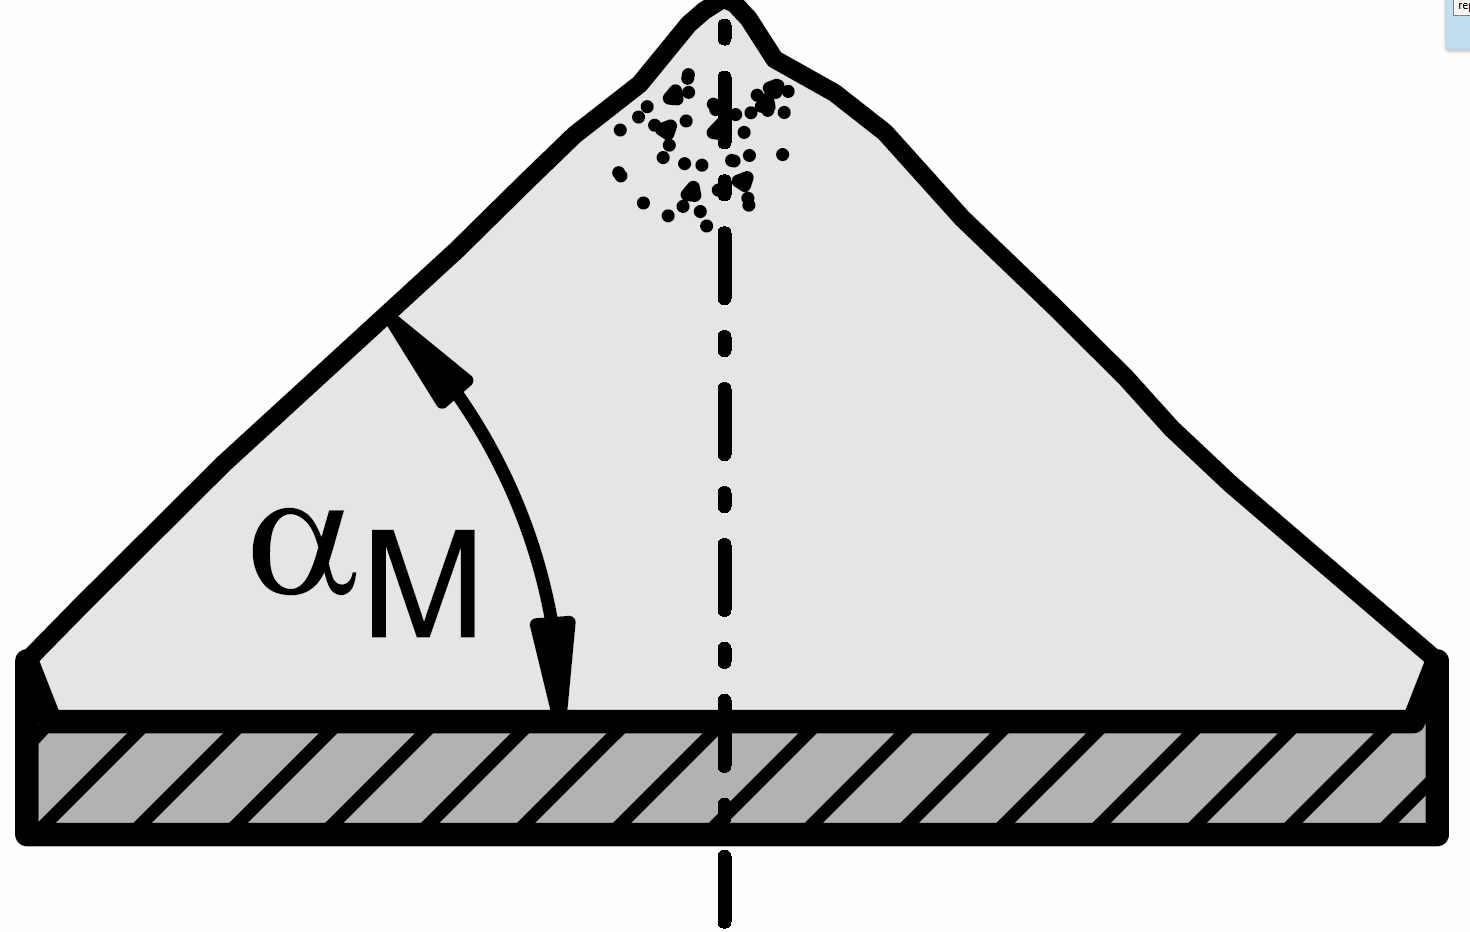
\includegraphics[width=.40\columnwidth]{images/005aor}
	  \label{fig:005aor}
  }
  \\
  \caption{AoR experimental tester.}
  \label{fig:088aorexperimental}
\end{figure}
\info{decide if putting the complete table}
\begin{table}[h!]
\centering
\begin{tabular}{ll|cc}
\hline
          &       & \multicolumn{2}{c}{AOR $[^\circ]$} \\
            & scale & small & large \\
\hline
    coke  & coarse & 40.90 & \\
      & fine  & 42.60 &  \\
\hline      
    iron ore & coarse & 44.15 & 34.96 \\
     ore & fine  & 43.00 & \\
\hline     
    limestone & coarse & 37.75 & \\
     & fine  & 44.50 & \\
\hline     
    sinter & coarse & 39.05 & 35.81 \\
     & fine  & 38.85 & \\
             \hline
\end{tabular}
\caption{AOR experimental values.}
\label{tab:23aor}
\end{table}

\section{Drained angle of repose (p-p) - large scale}
\label{sec:aorlargescale}

\info{decide if keeping}
At the Leoben VAS facility a new rotating double chute was used: 
nine large scale dynamic angle of repose tests were performed. 
\improvement{Evaluate large-small scale AoR relationship and put some images.}

\section{Jenike Shear Cell tester}
\label{sec:jsct}
%************************************************

The third step of the procedure was using shear testers - 
a simplified Jenike shear cell tester (\acs{JSCT}, Fig. \ref{fig:003sjsct}, see
\citet{RefWorks:114}) and a Schulze ring shear cell
tester (\acs{SCT}, see \citet{RefWorks:142}) to characterize particle flow
properties, especially the complete yield locus.
Compared to the original \acs{JSCT} in Fig. \ref{fig:052ShearCellLab}, we
defined our tester in Fig.
\ref{fig:053PoorMan} simplified because it is a prototype designed for fast characterization (see \citet{RefWorks:138}).
Each experiment was performed on a fresh material sample. \\
In the tests with the simplified \acs{JSCT}, a representative sample of bulk solid 
was placed in a shear cell of 104 millimiters diameter. 
This specimen was pre-consolidated by twisting the shear cell cover while applying a 
compressive load (from 0.488 to 1.379 kg) normal to it.\\
Since this was a simplified tester, the specimen was then sheared with the 
same normal load at a constant velocity. 
In fact, the \textit{shear to failure} phase was missing in these \textit{simplified} tests, 
and the \textit{consolidation} phase was not completely serialized.
The steady-state flow horizontal stress (Fig. \ref{fig:004sjsctdiagram}) is
called pre-shear stress ($\tau_{psh}$). 
Knowing the normal stress, it gives (Eq. \ref{eq:phi_ps}) the angle of internal 
friction of the pre-shear phase ($\phi_{e-psh}$), our first flowability value \cite{RefWorks:118}:
%************************************************
\begin{equation}
\begin{aligned}
\phi_{e-psh} &= \arctan \left(\frac{\tau_{psh}}{\sigma_{n,psh}} \right) ,\\
\mu_{psh} &=\tan(\phi_{e-psh}) .
\end{aligned}
 \label{eq:phi_ps}
\end{equation}

%************************************************
\begin{figure}[htbp]
\centering 
  \subfloat[Jenike shear cell tester.]{
	  \includegraphics[width=.44\columnwidth]{images/052ShearCellLab}
	  \label{fig:052ShearCellLab}
  }
  \quad
    \subfloat[Simplified Jenike shear cell tester.]{
	  \includegraphics[width=.44\columnwidth]{images/053PoorMan}
	  \label{fig:053PoorMan}
  }
  \\
  \subfloat[Jenike shear cell tester layout \cite{RefWorks:69}.]{
	  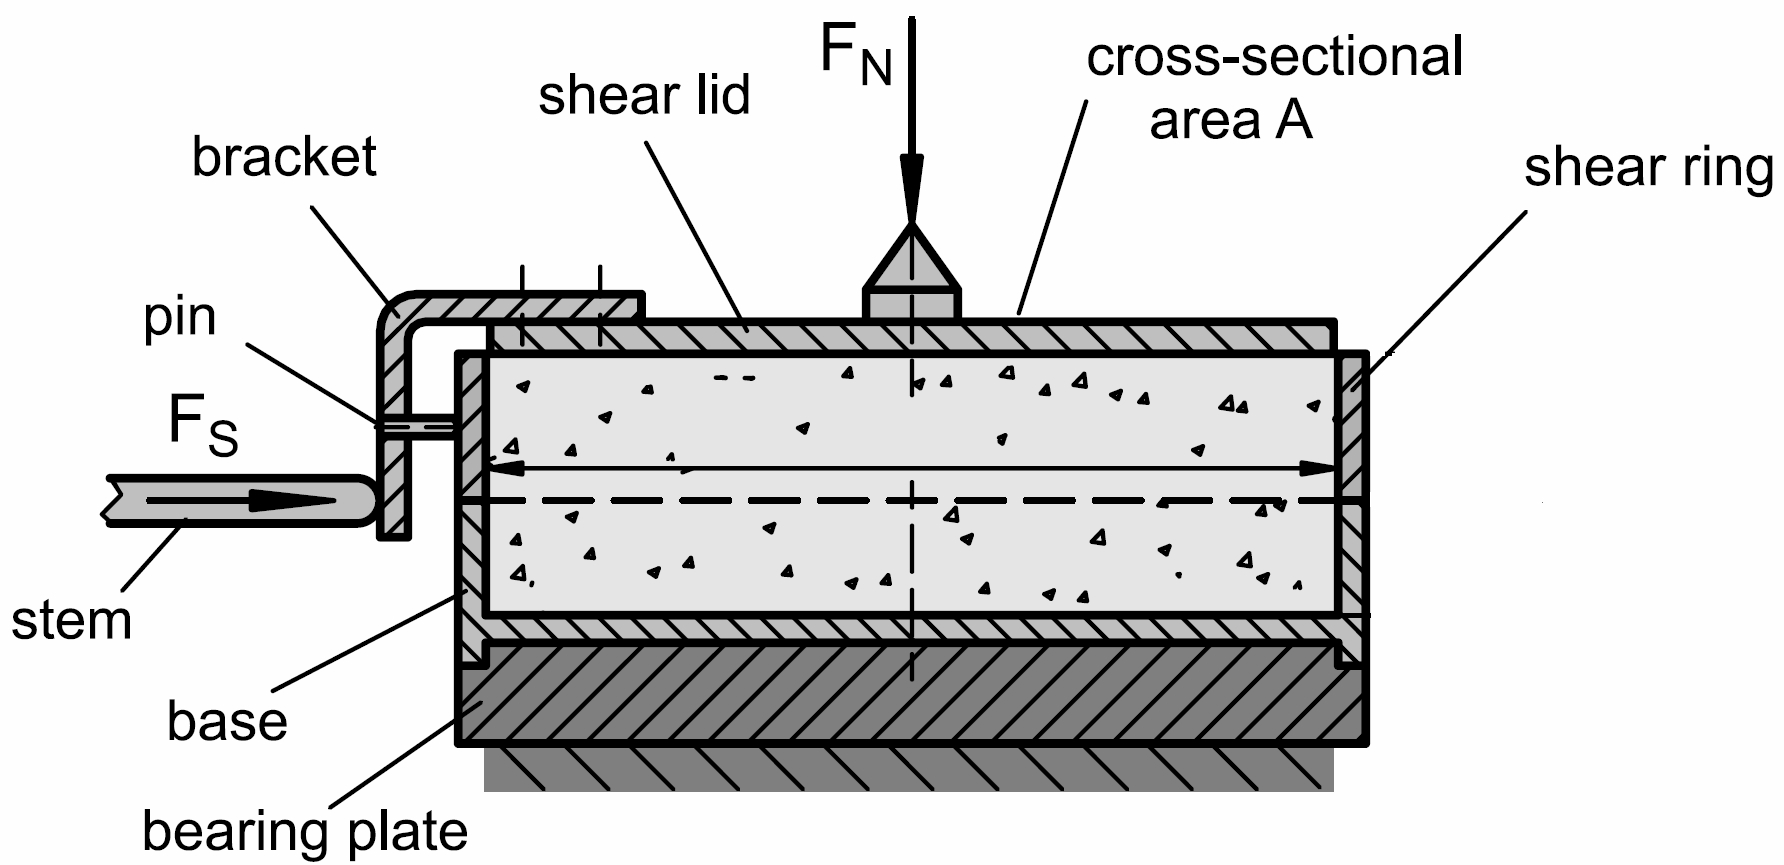
\includegraphics[width=.44\columnwidth]{images/003sjsct}
	  \label{fig:003sjsct}
  }
  \quad
    \subfloat[Jenike shear cell tester diagram \cite{RefWorks:69}.]{
	  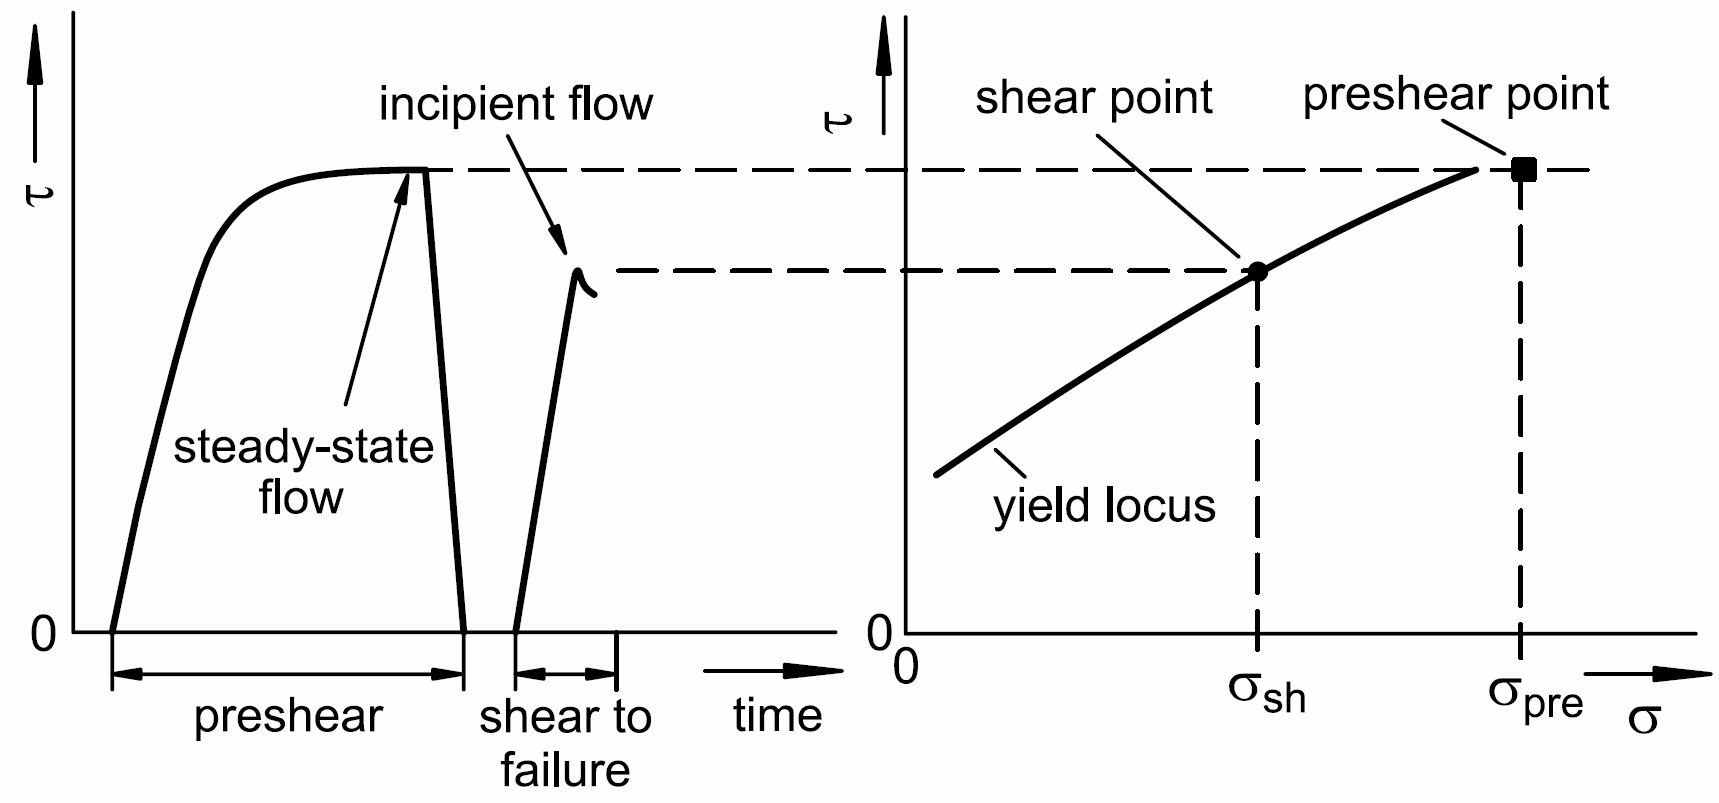
\includegraphics[width=.44\columnwidth]{images/004sjsctdiagram}
	  \label{fig:004sjsctdiagram}  }
  \\
  \caption{JSCT.}
  \label{fig:089jsctexperimental}
\end{figure}
The values obtained in the tests are summarized in Table \ref{tab:24shearcell4}.

\begin{sidewaystable}%[h]
\centering
\begin{tabular}{ll|ccccccccccccccc}
\hline
    normal & stress [Pa] & 562   & 562   & 562   & 562   & 562   & 1026  & 1026  & 1026  & 1026  & 1026  & 1588  & 1588  & 1588  & 1588  & 1588 \\
\hline 
          & test  & 1     & 2     & 3     & 4     & 5     & 6     & 7     & 8     & 9     & 10    & 11    & 12    & 13    & 14    & 15 \\
\hline
    coke  & coarse & 0.880 & 0.853 & 0.894 & 0.927 & 0.872 & 0.924 & 0.818 & 0.860 & 0.931 & 0.928 & 0.906 & 0.876 & 0.853 & 0.849 & 0.850 \\
      & fine  & 0.827 & 0.821 & 0.969 & 0.780 & 0.868 & 0.725 & 0.754 & 0.870 & 0.922 & 0.700 & 0.675 & 0.839 & 0.654 & 0.814 & 0.757 \\
\hline
    iron ore & coarse & 1.906 & 2.140 & 1.928 & 2.129 & 1.659 & 1.534 & 1.432 & 1.488 & 1.519 & 1.486 & 1.343 & 1.403 & 1.342 & 1.193 & 1.385 \\
     ore & fine  & 1.872 & 1.857 & 1.770 & 1.957 & 1.894 & 1.284 & 1.326 & 1.573 & 1.502 & 1.736 & 1.403 & 1.379 & 1.220 & 1.378 & 1.156 \\
\hline
    limestone & coarse & 1.257 & 1.108 & 1.349 & 1.305 & 1.306 & 1.010 & 0.887 & 0.909 & 0.884 & 0.880 & 0.718 & 0.749 & 0.819 & 0.859 & 0.824 \\
     & fine  & 1.443 & 1.197 & 1.199 & 1.328 & 1.335 & 1.074 & 0.934 & 0.959 & 1.069 & 0.909 & 0.876 & 0.862 & 0.867 & 0.898 & 0.949 \\
\hline
    sinter & coarse & 1.098 & 1.056 & 1.296 & 1.368 & 1.362 & 1.014 & 1.299 & 1.057 & 1.131 & 0.990 & 0.895 & 0.996 & 0.971 & 0.975 & 0.744 \\
         \hline
\end{tabular}
\caption[JSCT experimental values]{\acs{JSCT} experimental values.
Coefficients of internal frictions in different load conditions.}
\label{tab:24shearcell4}
\end{sidewaystable}

\section{Schulze Ring Shear Cell tester (p-p)}
\label{sec:SRSCT}
%************************************************
\begin{figure}[htbp]
\centering 
  \subfloat[SCT.]{
	  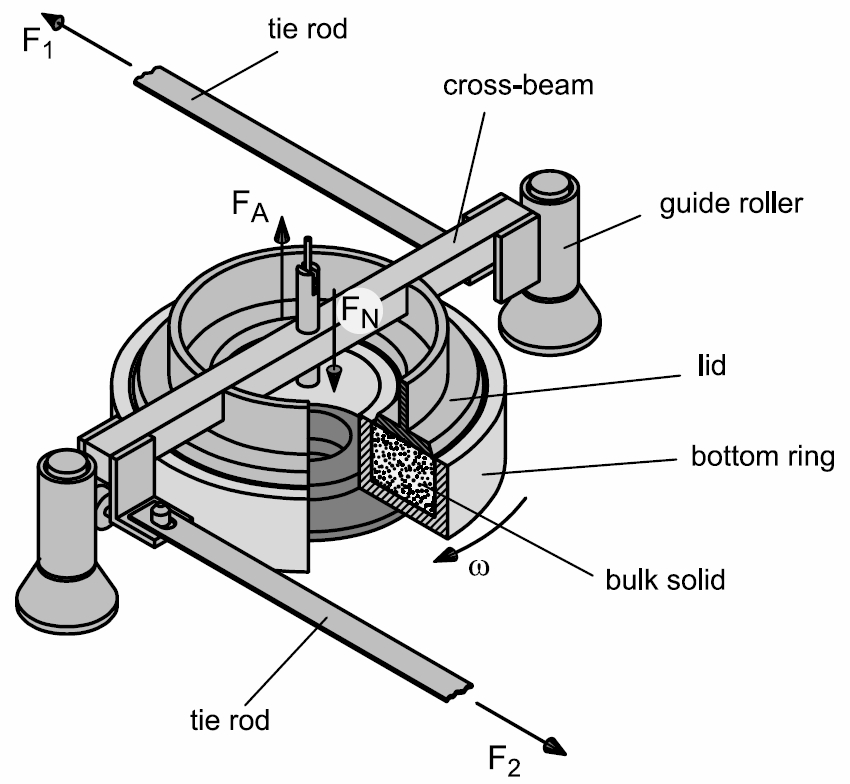
\includegraphics[width=.40\columnwidth]{images/001srsct}
	  \label{fig:001srsct}
  }
  \quad
    \subfloat[SCT diagram.]{
	  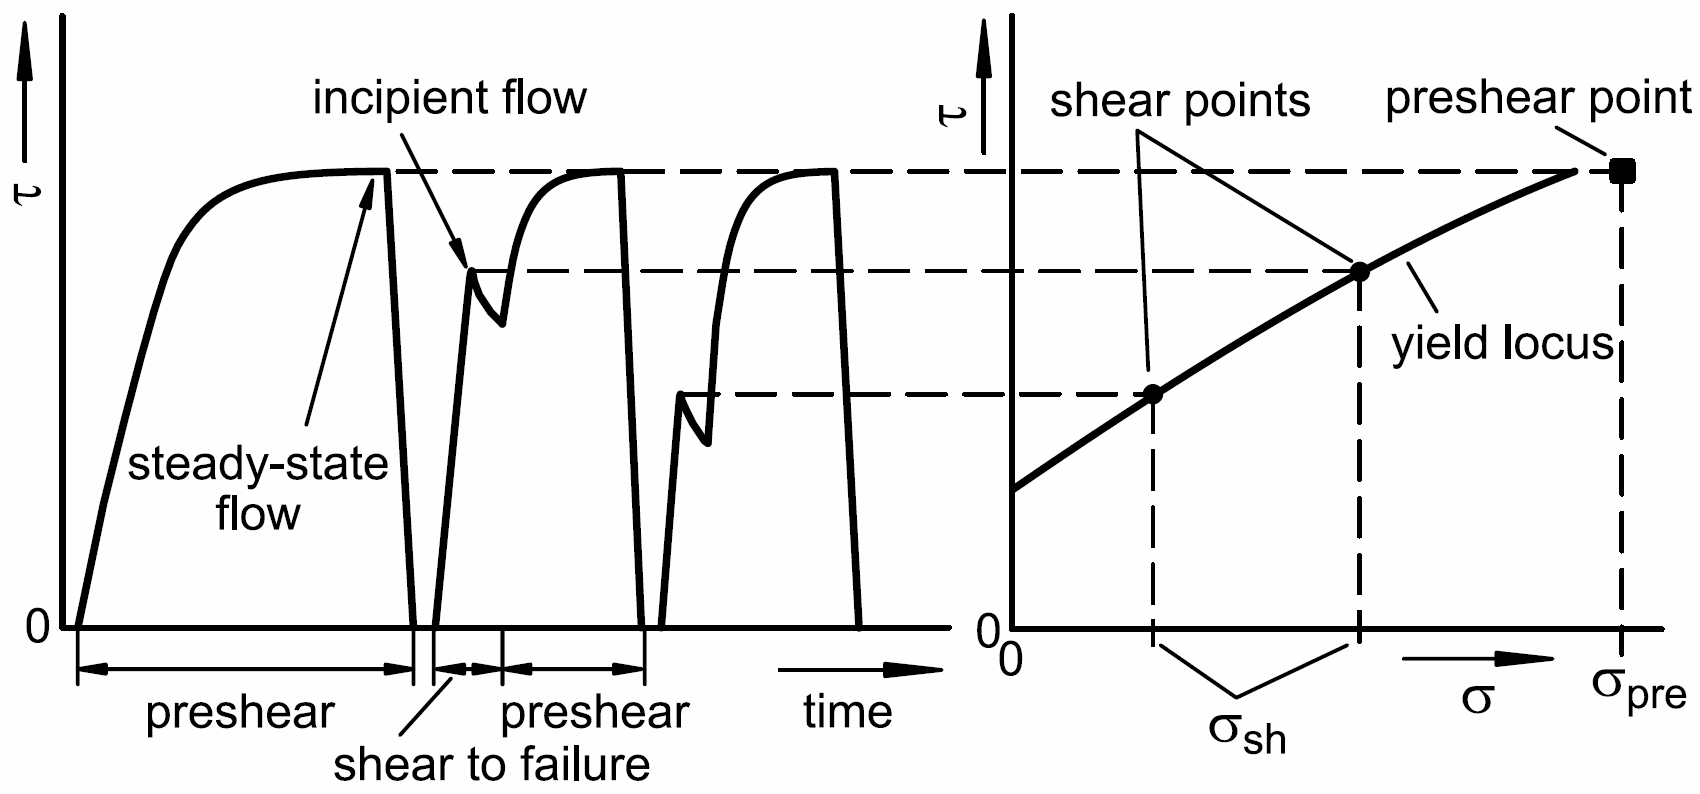
\includegraphics[width=.54\columnwidth]{images/002srsctdiagram}
	  \label{fig:002srsctdiagram}
  }
  \\
  \caption{SCT experimental tester.}
  \label{fig:090sctexperimental}
\end{figure}

A representative sample of bulk solid was placed in a Schulze ring shear cell
tester (\acs{SCT}) of specified dimensions ($external ~ radius = 100 ~ mm$,
$internal ~ radius = 50 ~ mm$), see Fig. \ref{fig:001srsct}.

\subsection{SRSCT procedure}
\label{subsec:srsctprocedure}

A normal load was applied to the cover. As soon as the lid touched the sample,
its position was calculated.
Together with the area of the ring, the total volume can be calculated, and subsequently the 
\textit{bulk density} \acs{rhob}:
%************************************************
\begin{equation}
\rho_b = \frac{mass}{volume}.
 \label{eq:rhob}
\end{equation}

%************************************************
\begin{figure}[!htb] 
\centering 
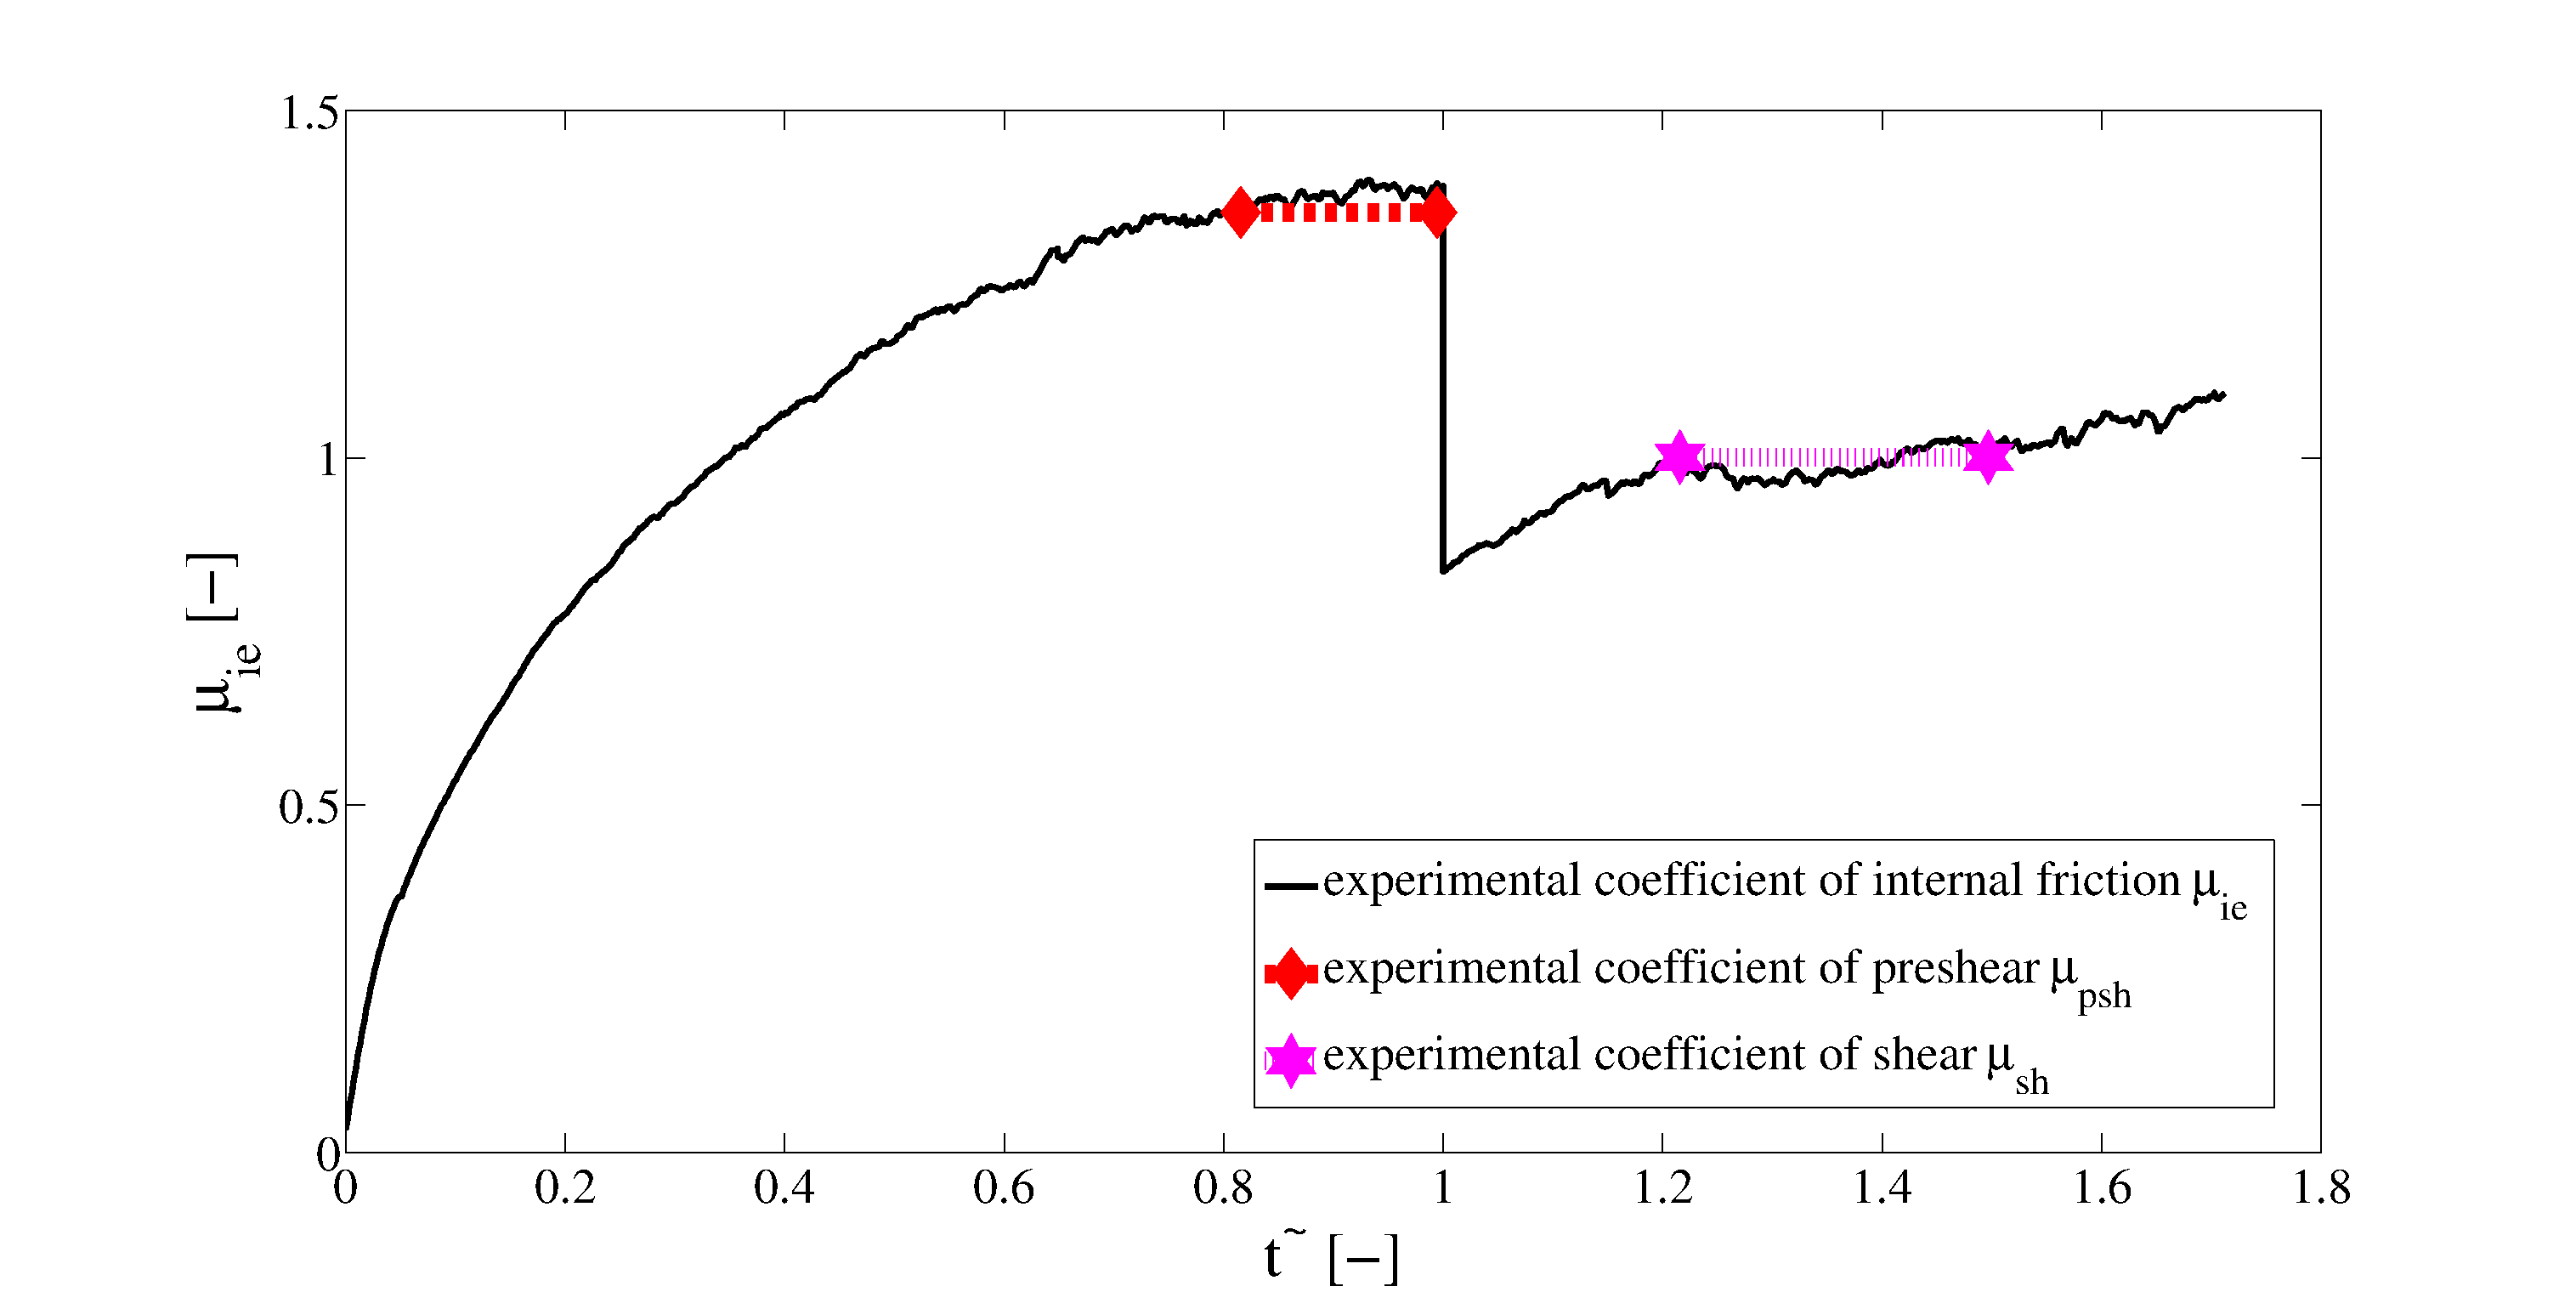
\includegraphics[width=.96\textwidth]{images/020experimental} 
\caption[Experimental shear cell tester stress path]{Experimental shear-cell tester stress path - $\sigma_n = 10000
        ~Pa$.}
\label{fig:020experimental} 
\end{figure}

% \begin{figure}[htp] \centering
%     \begin{subfigure}[b]{0.96\columnwidth}
%         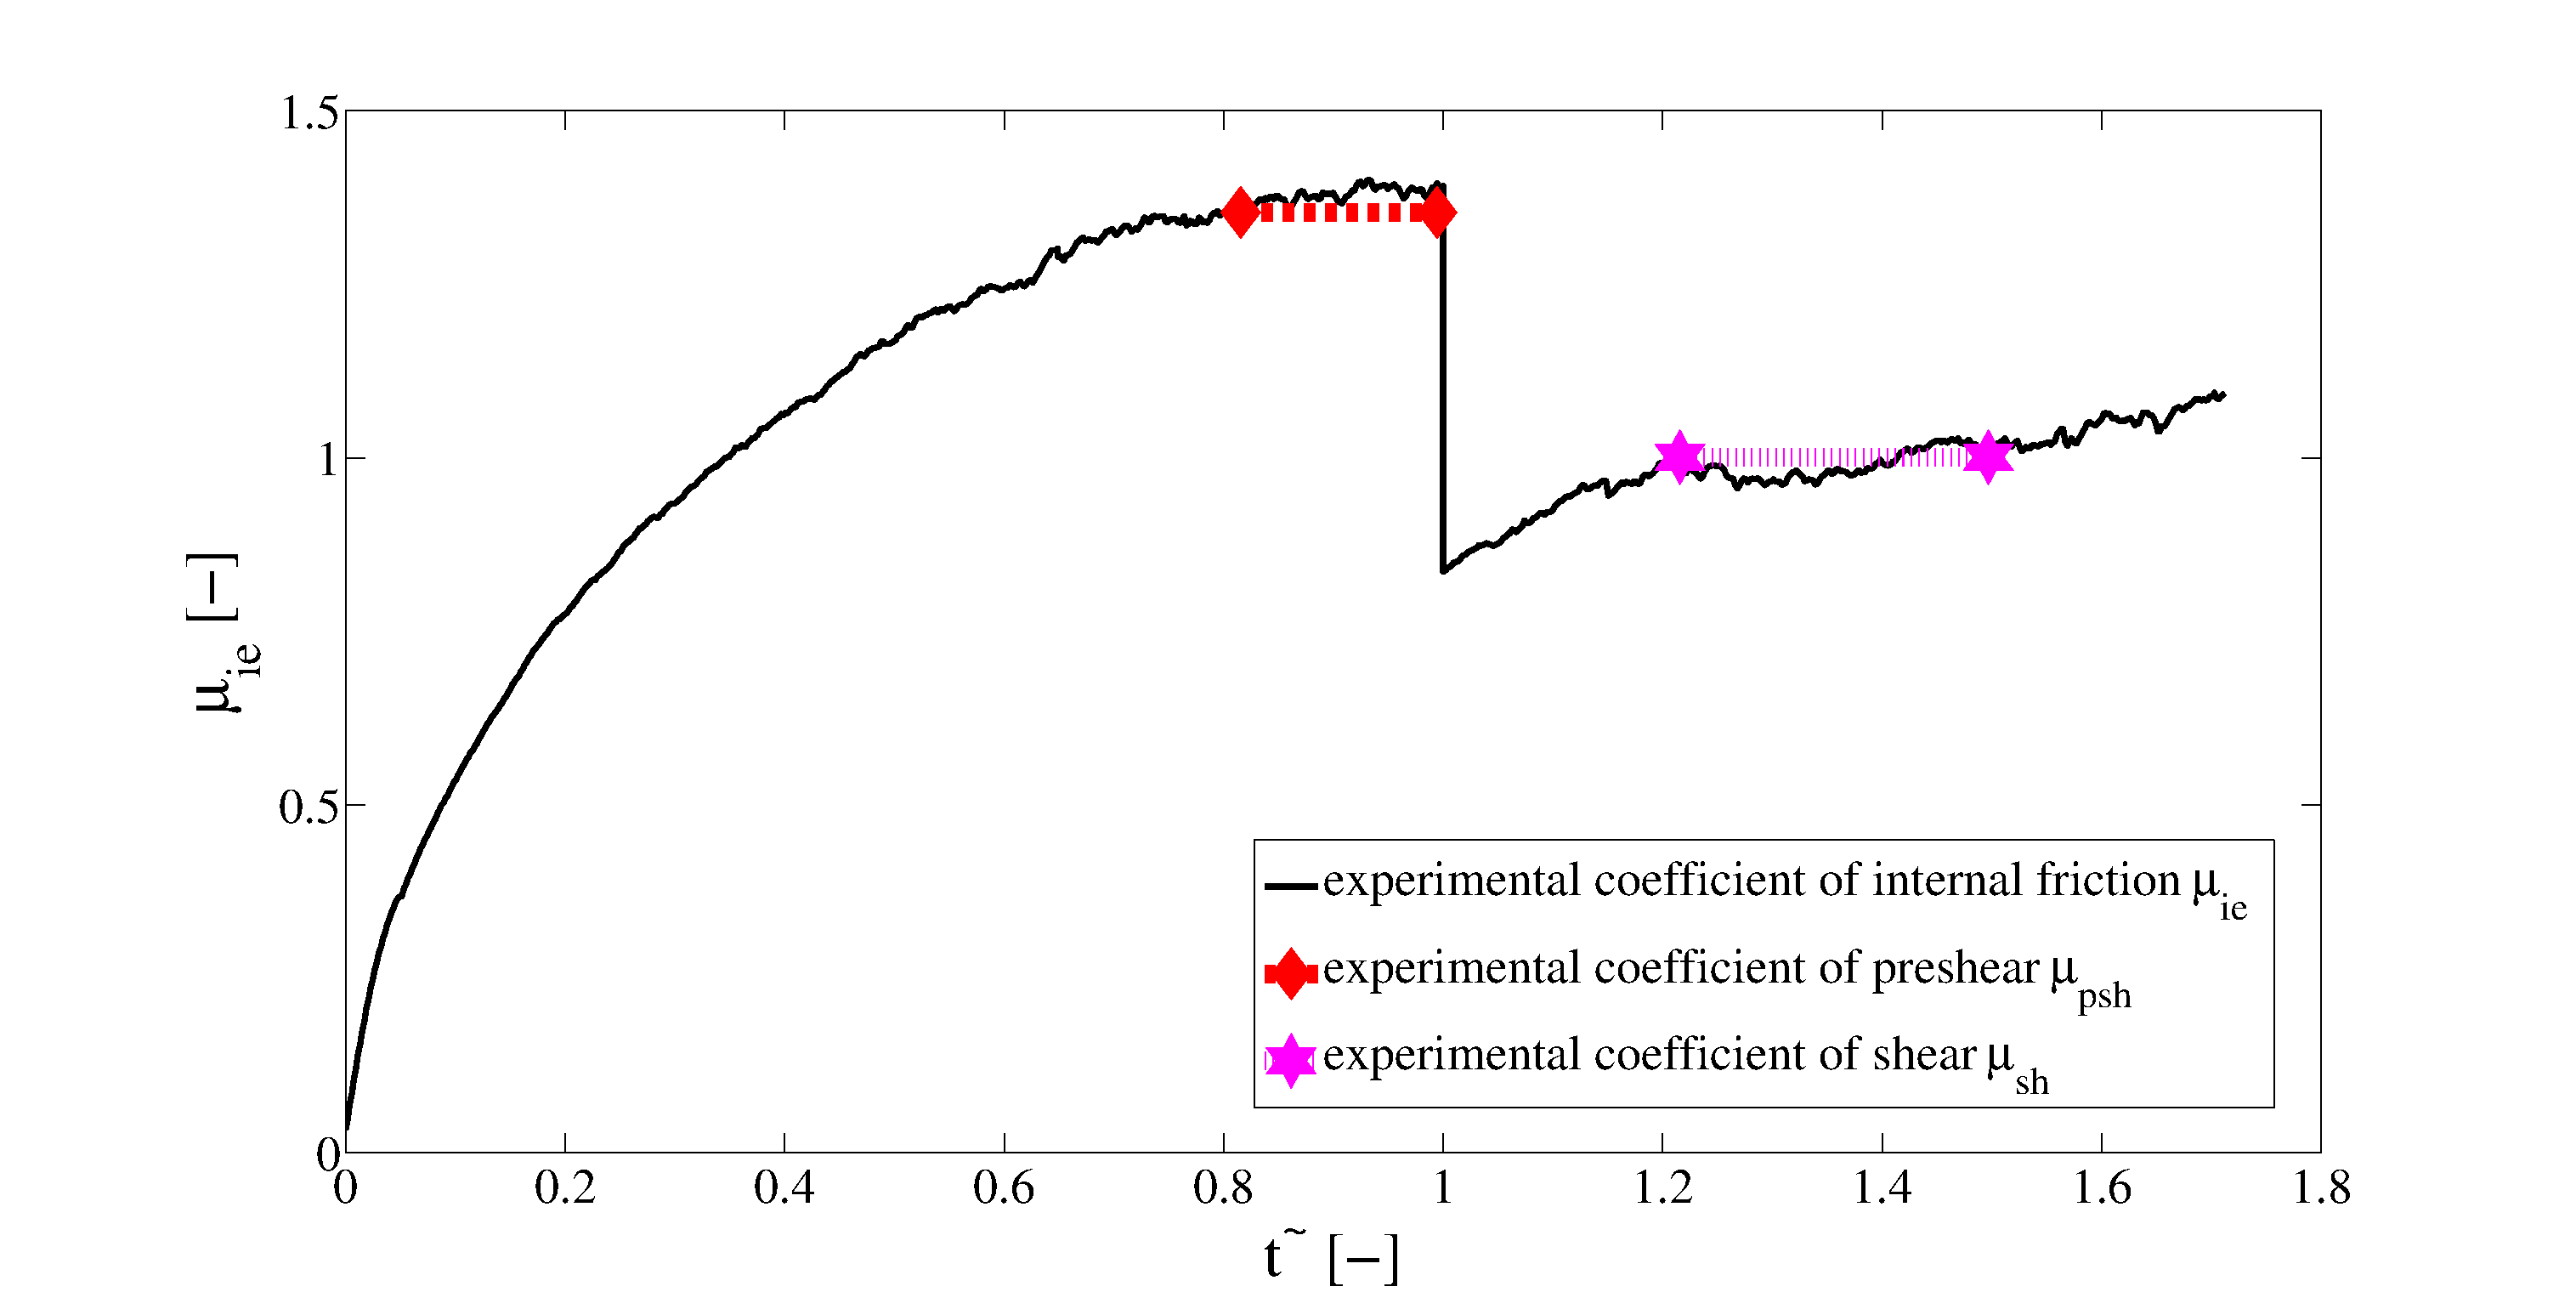
\includegraphics[width=\textwidth]{20experimental}
%         \caption{Experimental shear-cell tester stress path - $\sigma_n = 10000
%         ~Pa$}
%         \label{fig:20experimental} 
%     \end{subfigure}\\
%         \begin{subfigure}[b]{0.96\columnwidth}
%         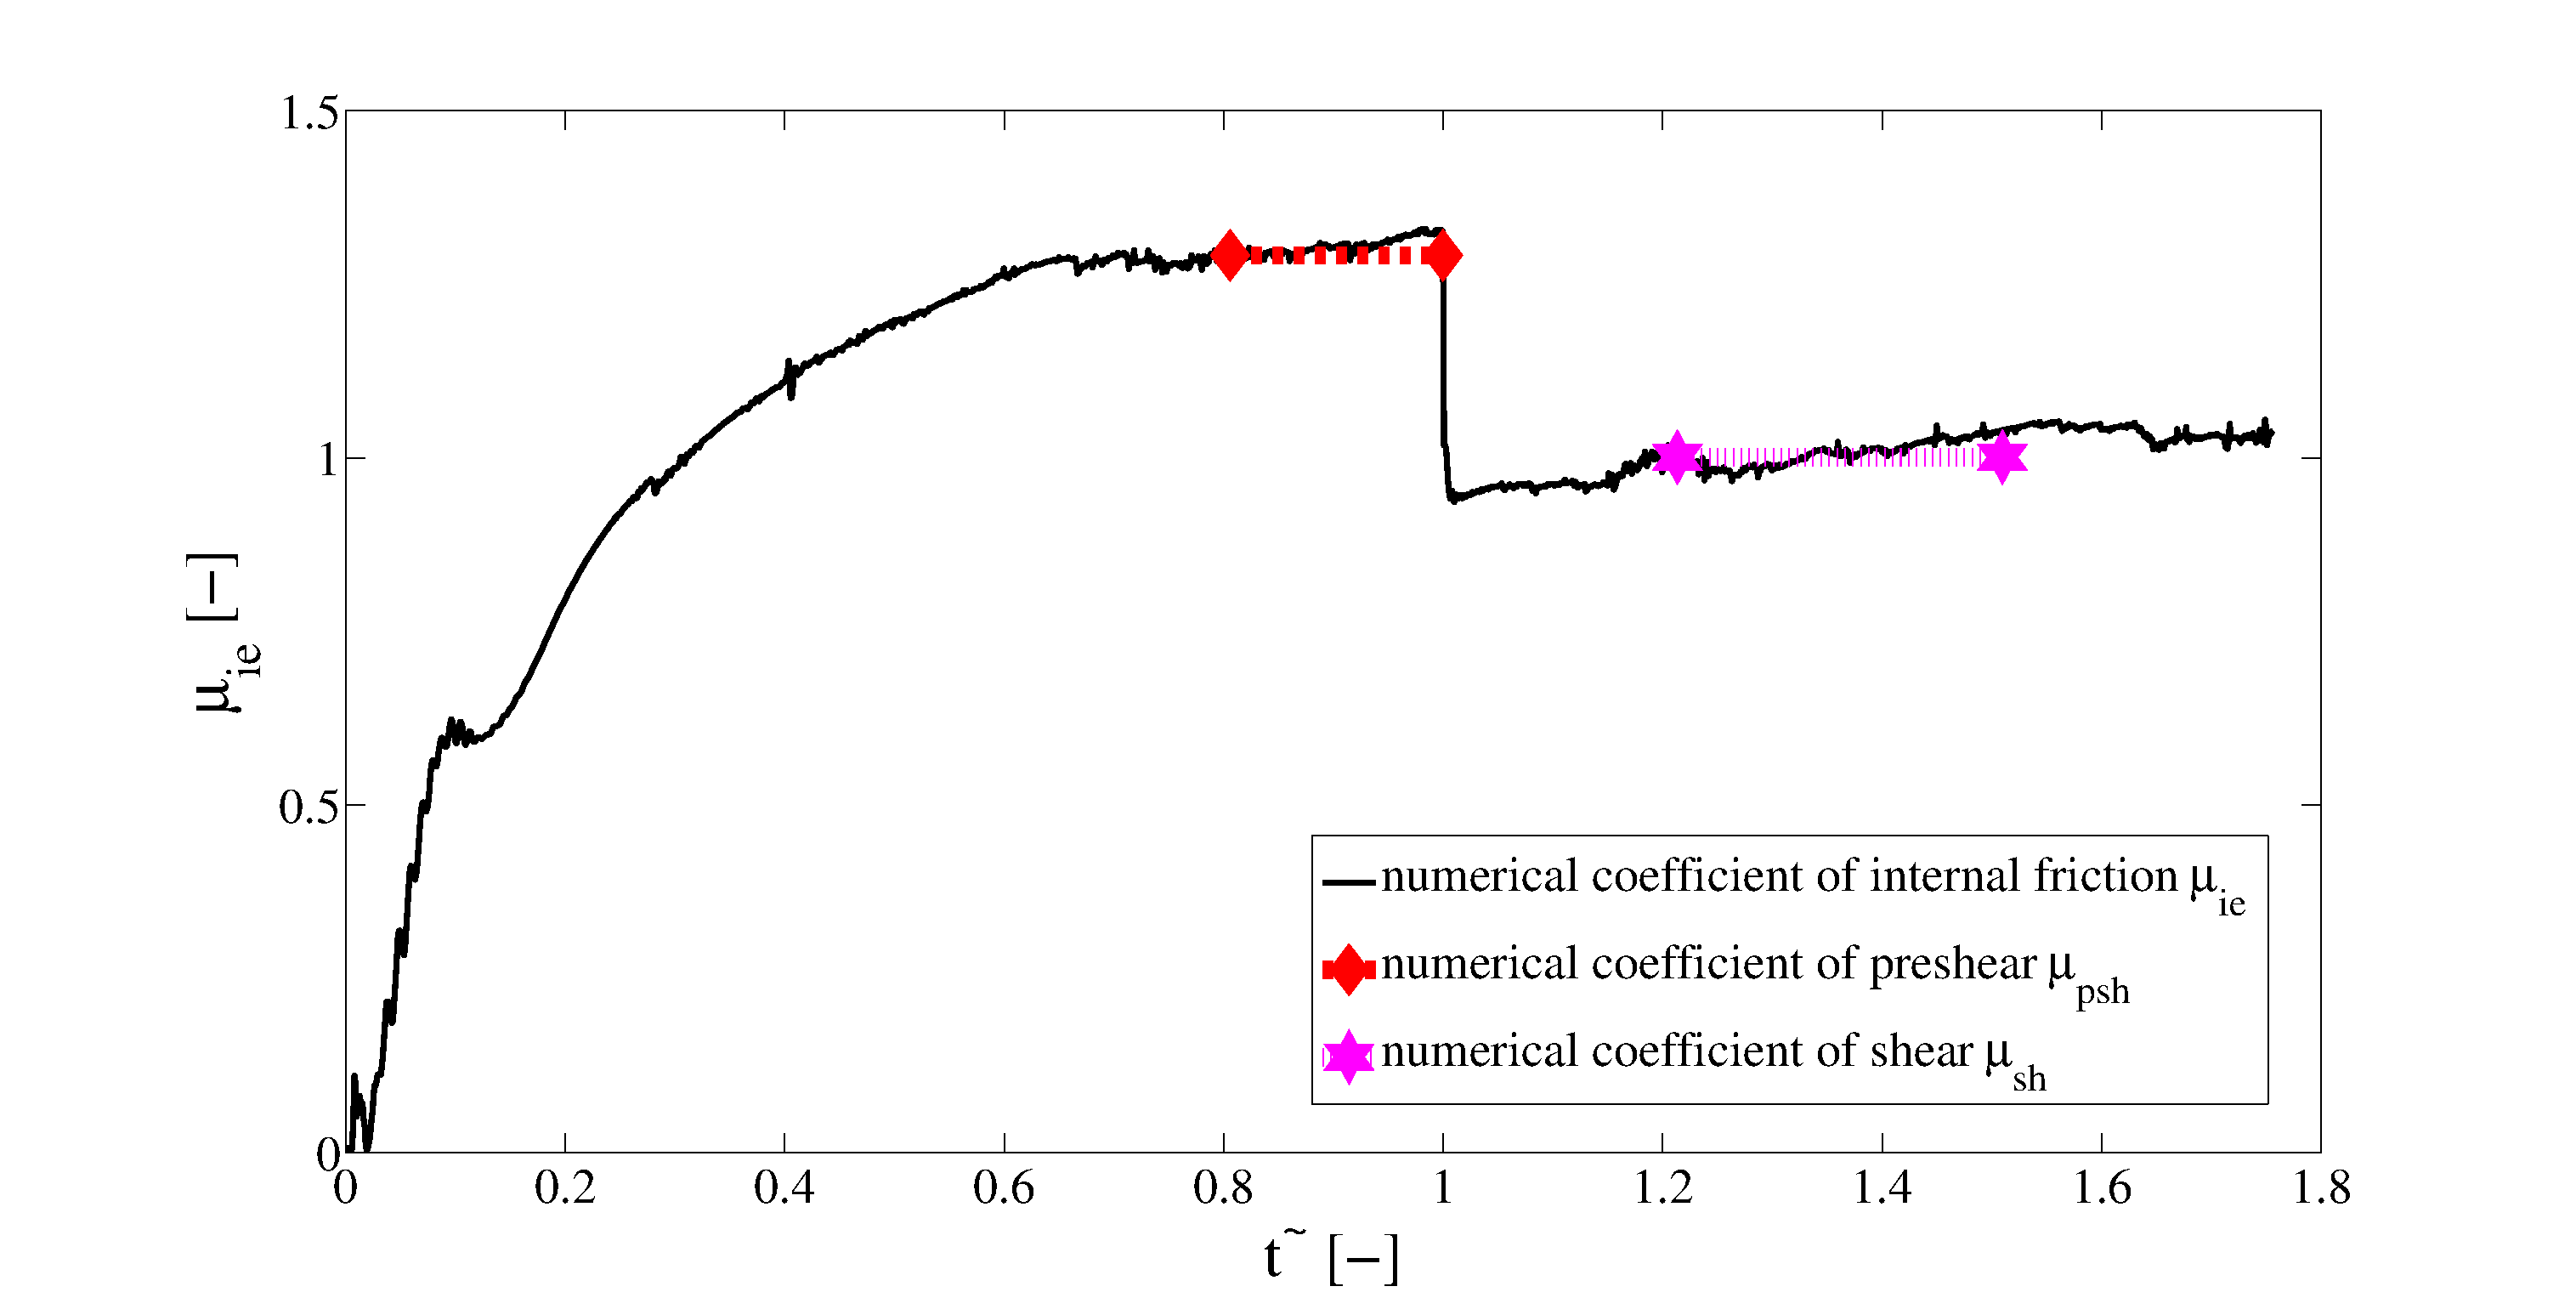
\includegraphics[width=\textwidth]{21simexample}
%         \caption{Numerical shear-cell tester stress path - $\sigma_n = 10000
%         ~Pa$}
%         \label{fig:21simexample} 
%     \end{subfigure}
%     \caption[Stress path]{Experimental and numerical samples of the stress path
%     for the Schulze ring shear cell tester.
% 	Time was normalized: $\tilde{t} = t/t_{change}$, where $t_{change}$ is the
% 	point in time at which the normal stress (\acs{sigman}) was modified during the
% 	tests.
% 	Until $\tilde{t}=1$, the \acs{sigman} was kept constant at 10,000 Pa. 
% 	In Fig. \ref{fig:20experimental}, 
%  	a plateau was reached at $\tilde{t}~=0.91$.
% 	The coefficient of pre-shear (\acs{mupsh}) was calculated as the average of the
% 	coefficient of internal friction (\acs{muie}) in this first plateau.
% 	At $\tilde{t}=1$, the \acs{sigman} was reduced to $80 \%$ of its initial
% 	value, and soon after
% 	a second plateau developed.
% 	We obtained the coefficient of
% 	shear ($ \mu_{sh}$) as the average of \acs{muie} in this second plateau.
% 	The stress paths agree well, especially the plateaux.
% 	They were clearly relevant because
% 	the values representative of the bulk behaviours 
% 	were collected there.}
%     \label{fig:40experimentalsimulation}
% \end{figure}
the first bulk value
of the sample, was obtained.
Later, we tried to obtained the \textit{bulk values} indicated in Table
\ref{tab:14bulkvalues}, slightly different from those indicated in Fig.
\ref{fig:002srsctdiagram}.\\
A representative stress path can be seen in Fig. \ref{fig:020experimental}.
Time was normalized: $\tilde{t} = t/t_{change}$, where $t_{change}$ is the
point in time at which the normal stress (\acs{sigman}) was modified during the	tests.
After the \acs{rhob} identification, the \acs{sigman} was kept constant at e.g.
10,000 Pa until $\tilde{t}=1$.
The specimen was in this way pre-sheared until a steady-state shear value was
reached from $\tilde{t}~=0.91$ to $\tilde{t}=1$.
The steady-state flow horizontal stress
is called steady-state flow/pre-shear stress.
If the normal stress is known, it provides (Eq. \ref{eq:phi_ps}) the angle of
internal friction of the pre-shear phase ($\phi_{e-psh}$), and consequently the
pre-shear coefficient of internal friction $ (\mu_{psh})$, the second
bulk value, see \citet{RefWorks:118}, see Eq. \ref{eq:phi_ps}.\\
At $\tilde{t}=1$ the normal stress and the angular velocity were then
immediately reduced to zero.
Subsequently, the specimen was sheared under a fraction (\acs{tauperc})(e.g.
80\%) of the first normal load until the shear force reached a a second plateau.
Both the pre-shear and shear phases were executed at constant velocity. 
We define the horizontal stress at the shear force peak as the average shear
stress in this second plateau, thus obtaining the incipient flow/shear
coefficient of internal friction \acs{mush}, third bulk value (Eq. \ref{eq:phi_s})\cite{RefWorks:118}:
%************************************************
\begin{equation}
\begin{aligned}
\phi_{e-sh} &= \arctan \left(\frac{\tau_{sh}}{\sigma_{n,sh}} \right) ,\\
\mu_{sh} &= \tan(\phi_{e-sh}) .
\end{aligned}
 \label{eq:phi_s}
\end{equation}

%************************************************
Between two and five different pre-shear normal loads were applied in each
experiment (1,000, 2,000, 5,000, 10,000, and 15,000 Pa).
For each we used a normal load proportional to the initial one
(\acs{tauperc}), increasing from stage one (40\%) to stage four (100\%)
with two escalating intermediate stages (60\% and 80\%).
Each experiment was performed on a fresh material sample. \\

\subsection{SRSCT results}
\label{subsec:srsctresults}

The tipical stress path, normalized into coefficient of internal friction on the
y-axis and normalized time on the x-axis, can be seen in Fig.
\ref{fig:020experimental}.\\
We then collected the results of the 26 tests performed according to the load
conditions of Table \ref{tab:21shearcell2} in Tables \ref{tab:20shearcell1}
and \ref{tab:22shearcell3}.
Each of the four column represents one load stage.
Further, $\rho_{b-100}$ has been used as bulk value $\rho_{b}$.
Intuitevely, $\phi_{e-100}$ was the $\phi_{e-psh}$, while $\phi_{e-40}$,
$\phi_{e-60}$, and $\phi_{e-80}$ represented the $\phi_{e-sh}$ in the different
stages.
The experimental values collected were used for the identification of the
microscopic numerical parameters (further details in Chapter
\ref{cap:anntraining}).
\begin{table}%[h]
\centering
\begin{tabular}{ll|c|cccc|cccc}
\hline
          &       & test  & $\sigma_{Ab40}$ & $\sigma_{Ab60}$ & $\sigma_{Ab80}$ &
          $\sigma_{Ab100}$ & $\tau_{Ab40}$ & $\tau_{Ab60}$ & $\tau_{Ab80}$ &
          $\tau_{Ab100}$ \\
\hline          
    coke  & coarse & 1     & 819   & 1221  & 1621  & 2020  & 1246  & 1376  & 1551  & 1841 \\
          &       & 2     & 2020  & 3021  & 4020  & 5020  & 2296  & 3243  & 3853  & 4486 \\
\hline
    coke  & fine  & 1     & 828   & 1230  & 1629  & 2029  & 1154  & 1418  & 1726  & 1819 \\
          &       & 2     & 2030  & 3031  & 4029  & 5030  & 2347  & 3079  & 3778  & 4064 \\
          &       & 3     & 4030  & 6032  & 8031  & 10031 & 4261  & 6028  & 7367  & 7939 \\
\hline
    iron ore & coarse & 1     & 884   & 1286  & 1686  & 2085  & 1954  & 1687  & 2092  & 2173 \\
          &       & 2     & 4086  & 6088  & 8088  & 10087 & 4507  & 6083  & 6990  & 8375 \\
          &       & 3     & 2087  & 3088  & 4087  & 5087  & 2524  & 5098  & 4273  & 4606 \\
\hline
    iron ore & fine  & 1     & 488   & 689   & 888   & 1090  & 594   & 755   & 939   & 1027 \\
          &       & 2     & 887   & 1288  & 1687  & 2087  & 1248  & 1449  & 1800  & 1948 \\
          &       & 3     & 2092  & 3093  & 4092  & 5092  & 2285  & 3084  & 3956  & 4343 \\
          &       & 4     & 4094  & 6096  & 8096  & 10095 & 4830  & 6442  & 7820  & 8805 \\
          &       & 5     & 6093  & 9091  & 12091 & 15092 & 6705  & 9640  & 11797 & 12885 \\
\hline
    limestone & coarse & 1     & 849   & 1251  & 1650  & 2050  & 1525  & 1946  & 1679  & 1718 \\
          &       & 2     & 2049  & 3050  & 4049  & 5050  & 2180  & 2952  & 3779  & 4193 \\
\hline
    limestone & fine  & 1     & 462   & 661   & 861   & 1063  & 673   & 853   & 957   & 1036 \\
          &       & 2     & 862   & 1264  & 1663  & 2063  & 1000  & 1326  & 1694  & 1841 \\
          &       & 3     & 2063  & 3064  & 4062  & 5063  & 2504  & 3225  & 4049  & 4449 \\
          &       & 4     & 4062  & 6064  & 8063  & 10063 & 4691  & 5977  & 7639  & 8609 \\
\hline
    sinter & coarse & 1     & 455   & 655   & 855   & 1056  & 591   & 722   & 734   & 751 \\
          &       & 2     & 857   & 1258  & 1657  & 2057  & 1153  & 1448  & 1554  & 1679 \\
          &       & 3     & 2058  & 3060  & 4058  & 5059  & 2479  & 2853  & 3419  & 4244 \\
\hline
    sinter & fine  & 1     & 467   & 667   & 866   & 1068  & 703   & 823   & 989   & 1059 \\
          &       & 2     & 868   & 1270  & 1669  & 2069  & 928   & 1371  & 1673  & 1818 \\
          &       & 3     & 2070  & 3070  & 4069  & 5070  & 2696  & 4322  & 3758  & 4352 \\
          &       & 4     & 4070  & 6071  & 8071  & 10070 & 4145  & 6729  & 9423  & 8232 \\
       \hline
\end{tabular}
\caption[SCT experimental values 2]{\acs{SCT} experimental values 2. Normal and
tangential stresses in different load conditions.}
\label{tab:21shearcell2}
\end{table}
\begin{table}%[h]
\centering
\begin{tabular}{ll|c|cccc|cccc}
\hline
          &       & test  & Dh40  & Dh60  & Dh80  & Dh100 & rhoB40 & rhoB60 & rhoB80 & rhoB100 \\
\hline          
    coke  & coarse & 1     & -0.542 & -0.302 & -0.09 & 0     & 516   & 519   & 522   & 519 \\
          &       & 2     & -1.329 & -0.941 & -0.838 & 0     & 518   & 523   & 524   & 521 \\
\hline 
    coke  & fine  & 1     & 4.136 & 4.166 & 4.089 & 0     & 738   & 739   & 737   & 738 \\
          &       & 2     & 5.465 & 5.361 & 5.253 & 0     & 771   & 769   & 766   & 769 \\
          &       & 3     & 5.284 & 5.214 & 5.067 & 0     & 787   & 786   & 782   & 785 \\
\hline 
    iron ore & coarse & 1     & -2.207 & -1.979 & -1.767 & 0     & 2176  & 2188  & 2200  & 2188 \\
          &       & 2     & -1.548 & -1.629 & -1.433 & 0     & 2225  & 2221  & 2231  & 2226 \\
          &       & 3     & -1.491 & -1.526 & -1.318 & 0     & 2227  & 2225  & 2236  & 2229 \\
\hline 
    iron ore & fine  & 1     & -0.893 & -0.74 & -0.784 & 0     & 2267  & 2276  & 2273  & 2272 \\
          &       & 2     & -0.696 & -0.742 & -0.86 & 0     & 2235  & 2232  & 2225  & 2231 \\
          &       & 3     & -0.042 & -0.059 & -0.051 & 0     & 2359  & 2358  & 2358  & 2358 \\
          &       & 4     & 0.318 & 0.317 & 0.344 & 0     & 2426  & 2426  & 2427  & 2426 \\
          &       & 5     & 0.829 & 0.753 & 0.805 & 0     & 2349  & 2344  & 2347  & 2347 \\
\hline 
    limestone & coarse & 1     & -2.693 & -2.746 & -2.669 & 0     & 1276  & 1275  & 1277  & 1276 \\
          &       & 2     & -2.183 & -2.032 & -1.95 & 0     & 1267  & 1272  & 1274  & 1271 \\
\hline 
    limestone & fine  & 1     & 0.059 & 0.045 & -0.069 & 0     & 1586  & 1586  & 1581  & 1584 \\
          &       & 2     & 0.599 & 0.518 & 0.442 & 0     & 1608  & 1605  & 1602  & 1605 \\
          &       & 3     & 1.424 & 1.412 & 1.308 & 0     & 1617  & 1617  & 1612  & 1615 \\
          &       & 4     & 1.359 & 1.318 & 1.162 & 0     & 1603  & 1602  & 1595  & 1600 \\
\hline 
    sinter & coarse & 1     & -2.637 & -2.661 & -2.708 & 0     & 1419  & 1418  & 1417  & 1418 \\
          &       & 2     & -2.081 & -2.145 & -2.249 & 0     & 1466  & 1464  & 1460  & 1463 \\
          &       & 3     & -3.268 & -3.076 & -3.236 & 0     & 1501  & 1508  & 1503  & 1504 \\
\hline 
    sinter & fine  & 1     & -2.002 & -1.909 & -1.958 & 0     & 1716  & 1720  & 1718  & 1718 \\
          &       & 2     & -1.001 & -1.014 & -1.082 & 0     & 1760  & 1760  & 1757  & 1759 \\
          &       & 3     & -0.568 & -0.617 & -0.656 & 0     & 1785  & 1783  & 1781  & 1783 \\
          &       & 4     & -0.025 & -0.038 & -0.115 & 0     & 1803  & 1803  & 1799  & 1802 \\
    \hline
\end{tabular}
\caption[aaaValid DEM values]{aaaValid DEM values. For each parameter we show
the valid parameter statistics in the two tests and in their intersection.
Finally, we show the number of valid parameter combinations over the total
(6250000).}
\label{tab:20shearcell1}
\end{table}
\begin{table}%[h]
\centering
\begin{tabular}{ll|c|cccc}
\hline
          &       & test  & $\phi_{ie-100}$ & $\phi_{ie-40}$ & $\phi_{ie-60}$ &
          $\phi_{ie-80}$ \\
\hline          
    coke  & coarse & 1     & 0.9114 & 1.4756 & 1.0724 & 1.0322 \\
          &       & 2     & 0.8936 & 1.1426 & 1.0568 & 0.9686 \\
\hline     
    coke  & fine  & 1     & 0.8965 & 1.3119 & 1.1963 & 1.0810 \\
          &       & 2     & 0.8080 & 1.1592 & 1.0200 & 0.9315 \\
          &       & 3     & 0.7914 & 1.0743 & 1.0127 & 0.8903 \\
\hline 
    iron ore & coarse & 1     & 1.0422 & 2.0971 & 1.3672 & 1.2524 \\
          &       & 2     & 0.8303 & 1.0771 & 0.9502 & 0.9270 \\
          &       & 3     & 0.9054 & 1.2179 & 1.6178 & 1.0593 \\
\hline 
    iron ore & fine  & 1     & 0.9422 & 1.1702 & 1.1140 & 1.0798 \\
          &       & 2     & 0.9334 & 1.4433 & 1.1321 & 1.0328 \\
          &       & 3     & 0.8529 & 1.0779 & 1.0013 & 0.9756 \\
          &       & 4     & 0.8722 & 1.1340 & 1.0805 & 0.9816 \\
          &       & 5     & 0.8538 & 1.1094 & 1.0640 & 0.9643 \\
\hline 
    limestone & coarse & 1     & 0.8380 & 1.8020 & 1.3885 & 1.1236 \\
          &       & 2     & 0.8303 & 1.0500 & 0.9866 & 0.9275 \\
\hline 
    limestone & fine  & 1     & 0.9746 & 1.4717 & 1.3099 & 1.0828 \\
          &       & 2     & 0.8924 & 1.2048 & 1.0380 & 0.9902 \\
          &       & 3     & 0.8787 & 1.2630 & 1.0419 & 0.9664 \\
          &       & 4     & 0.8555 & 1.1796 & 0.9890 & 0.9240 \\
\hline 
    sinter & coarse & 1     & 0.7112 & 1.2959 & 1.0868 & 0.8729 \\
          &       & 2     & 0.8162 & 1.3667 & 1.1486 & 0.9249 \\
          &       & 3     & 0.8389 & 1.1331 & 0.8827 & 0.9373 \\
\hline 
    sinter & fine  & 1     & 0.9916 & 1.4048 & 1.2185 & 1.2329 \\
          &       & 2     & 0.8787 & 1.0434 & 1.1084 & 0.9994 \\
          &       & 3     & 0.8584 & 1.2805 & 1.4067 & 0.9399 \\
          &       & 4     & 0.8175 & 1.0565 & 1.0635 & 1.1712 \\
         \hline
\end{tabular}
\caption[SCT experimental values 3]{\acs{SCT} experimental values 3.
Coefficients of internal frictions in the load conditions of Table
\ref{tab:21shearcell2}.}
\label{tab:22shearcell3}
\end{table}